\documentclass[aspectratio=169]{beamer}
\mode<presentation>

\title{digital plumbing}

\begin{document}
\begin{frame}
    \titlepage
\end{frame}

\begin{frame}{who am I?}
    \begin{description}[align=right]
        \setlength{\itemsep}{1cm}
        \item[undergrad:]
            \begin{itemize}
                \item BSc, Biomedical Engineering
                \item synthetic genomics/biology research advised by Jef Boeke
            \end{itemize}
        \item[currently:]
            \begin{itemize}
                \item PhD candidate, Biomedical Engineering
                \item research advised by Fred Winston
            \end{itemize}
    \end{description}
\end{frame}

\begin{frame}{grad school timeline}
\includegraphics[width=\textwidth]{figures/presentation_figure1-timeline.pdf}
\end{frame}

\begin{frame}{I develop analysis pipelines for genomics data}
\end{frame}

\begin{frame}{genomics data and its analysis are complex}
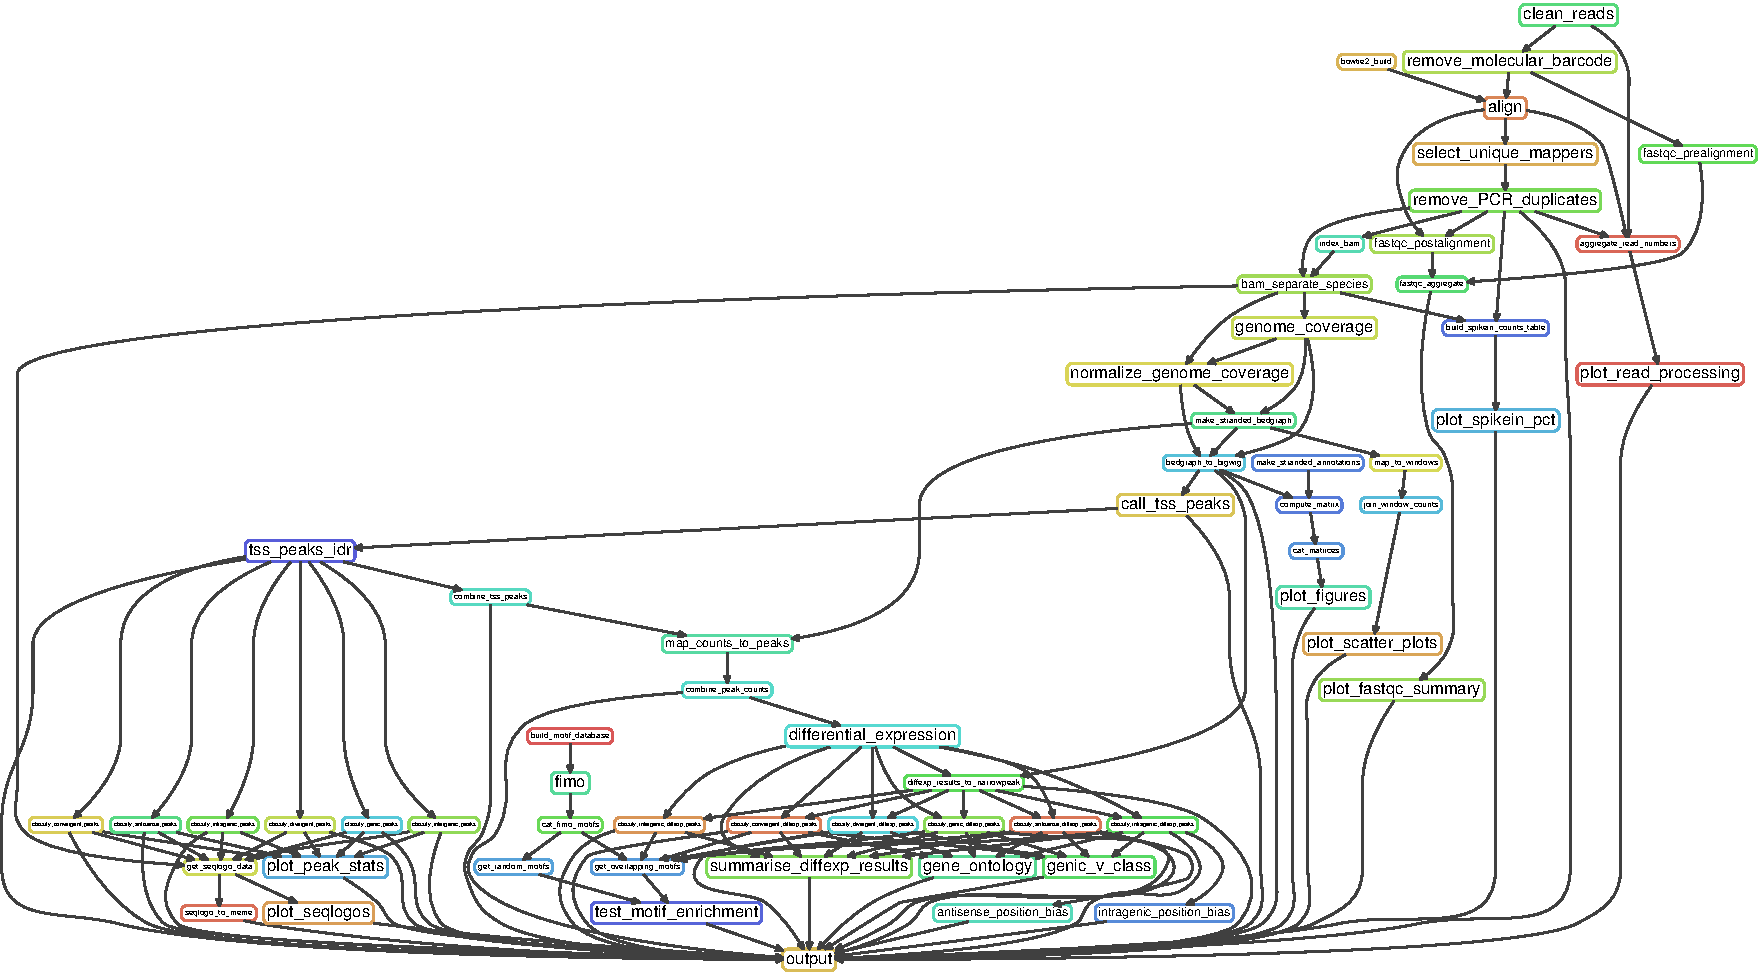
\includegraphics[width=\textwidth]{figures/rulegraph.pdf}
\end{frame}

\begin{frame}{Snakemake}
\end{frame}

\begin{frame}
    \begin{itemize}[]
        \setlength{\itemsep}{1cm}
        \item transcription elongation factor \textbf{Spt6}
        \item intragenic transcription in stress
        \item transcription elongation factor \textbf{Spt5}
    \end{itemize}
\end{frame}

\begin{frame}{intro to Spt6}
\end{frame}

\begin{frame}{Spt6 project collaborators}
    \begin{description}[align=right, noitemsep]
        \item [Steve Doris] optimized TSS-seq and ChIP-nexus protocols
        \item [] generated TSS-seq and ChIP-nexus libraries
        \item [Olga Viktorovskaya] generated MNase-seq libraries
        \item [Magdalenda Murawska] generated NET-seq libraries
        \item [Dan Spatt] wetlab experiments for publication
    \end{description}
\end{frame}

\begin{frame}{WASSDA}
\includegraphics[width=\textwidth]{figures/figure0_txn-diagram.pdf}
\end{frame}

% \begin{frame}
% \includegraphics[width=\textwidth]{figures/figure1_tss-seq-coverage.pdf}
% \end{frame}

% \begin{frame}
% \includegraphics[width=\textwidth]{figures/figure3_tfiib-nexus-tata.pdf}
% \end{frame}

\begin{frame}
\includegraphics[width=\textwidth]{figures/presentation_figure0-mvd1-coverage.pdf}
\end{frame}

\begin{frame}
\includegraphics[width=\textwidth]{figures/presentation_figure2_tss-seq-heatmaps.pdf}
\end{frame}

\begin{frame}
    \centering
    \includegraphics[height=0.2\textheight]{figures/figure0_txn-diagram.pdf}
    \begin{columns}
        \begin{column}{0.5\textwidth}
            \centering
            \includegraphics[width=\textwidth]{figures/presentation_figure6-tss-diffexp-summary.pdf}
        \end{column}
        \begin{column}{0.5\textwidth}
            \centering
            \pause
            \includegraphics[width=\textwidth]{figures/presentation_figure7-tss-expression-levels.pdf}
        \end{column}
    \end{columns}
\end{frame}

\begin{frame}
\centering
\includegraphics[width=\textwidth]{figures/presentation_figure3_tfiib-heatmaps.pdf}
\end{frame}

\begin{frame}{TFIIB is spread across the genome in \textit{spt6-1004}}
\includegraphics[width=\textwidth]{figures/figure8_tfiib-spreading-ssa4.pdf}
\end{frame}

\begin{frame}{new initiation explains most \textit{spt6-1004} intragenic transcripts}
    \centering
    \includegraphics[height=0.2\textheight]{figures/figure0_txn-diagram.pdf}
    \includegraphics[width=\textwidth]{figures/presentation_figure4_tss-v-tfiib.pdf}
\end{frame}

\begin{frame}{chromatin structure in \textit{spt6-1004}}
\includegraphics[width=\textwidth]{figures/presentation_figure9-mnase-metagene.pdf}
\end{frame}

\begin{frame}{quantifying changes in nucleosomes}
    \begin{columns}
        \begin{column}{0.5\textwidth}
            \centering
            \includegraphics[width=\textwidth]{figures/presentation_figure5-nucattributes.pdf}
        \end{column}
        \begin{column}{0.5\textwidth}
            \centering
            \includegraphics[width=\textwidth]{figures/presentation_figure8-global-nuc-fuzz-occ.pdf}
        \end{column}
    \end{columns}
\end{frame}

\begin{frame}
\includegraphics[width=\textwidth]{figures/presentation_figure10-mnase-heatmaps.pdf}
\end{frame}

\begin{frame}
\includegraphics[width=\textwidth]{figures/presentation_figure11-intragenic-mnase.pdf}
\end{frame}

\begin{frame}{intragenic promoters share features with genic promoters}
    \includegraphics[width=\textwidth]{figures/presentation_figure12-seqlogos.pdf}
\end{frame}

\begin{frame}{intragenic promoters share features with genic promoters}
    \includegraphics[width=\textwidth]{figures/presentation_figure13-intragenic-tata.pdf}
\end{frame}

\begin{frame}{functions of intragenic transcription project collaborators}
    \begin{description}[align=right, noitemsep]
        \item [Steve Doris] generated TSS-seq and ChIP-nexus libraries
        \item [Dan Spatt] polyribosome fractionation
    \end{description}
\end{frame}

\begin{frame}
\includegraphics[width=\textwidth]{figures/stress_figure1-tfiib-heatmaps.pdf}
\end{frame}

\begin{frame}{Spt5 project collaborators}
    \begin{description}[align=right, noitemsep]
        \item [Ameet Shetty] generated TSS-seq, MNase-seq, NET-seq, RNA-seq, and ChIP-seq libraries
    \end{description}
\end{frame}

\begin{frame}
\includegraphics[width=\textwidth]{figures/spt5_figure1-netseq-metagene.pdf}
\end{frame}

\begin{frame}
\includegraphics[width=\textwidth]{figures/spt5_figure2-rnaseq-heatmaps.pdf}
\end{frame}

\begin{frame}
\includegraphics[width=\textwidth]{figures/spt5_figure3-antisense-heatmaps.pdf}
\end{frame}

\begin{frame}
\includegraphics[width=\textwidth]{figures/spt5_figure4-mnase-metagene.pdf}
\end{frame}

\begin{frame}
\includegraphics[width=\textwidth]{figures/spt5_figure5-antisense-mnase-metagene.pdf}
\end{frame}

\end{document}
